\section{Описание метода решения}

Система разделена на два модуля: модуль сбора данных (Python) и модуль индексации/поиска (C++). Также дополнительно реализованы скрипты на Python для экспорта данных из MongoDB в текстовый файл и для визуализации закона Ципфа.

\subsection{Сбор данных}
В качестве корпуса были документов были выбраны спортивные новости на русском языке из kp.ru и sportrbc.ru.
Для сбора данных использовался поисковой робот на Python. 
Оба источника имеют удобные Sitemap-файлы, что значительно упростило навигацию по сайту и сбор ссылок на новости. 
Для каждого источника робот запускается в отдельном потоке и отправляет запрос на страницу из Sitemap 
с учетом задержки между запросами (2 секунды) для предотвращения блокировки. 
После получения HTML страницы с новостью, из нее извлекается контейнерный тег, содержащий только статью без элементов навигации, 
после чего загруженная статья сохраняется в MongoDB. 
Для простоты дальнейшей работы с данными используется скрипт, который экспортирует текущие данные из MongoDB в текстовый файл в следующем формате:
\begin{verbatim}
URL документа
Источник (новостной портал)
Заголовок статьи
Текст статьи
\end{verbatim}

Каждый документ занимает ровно 4 строки, что упрощает чтение и обработку данных в программе на C++.

\subsection{Индексация и Поиск}
Ядро поисковой системы написано на C++. В соответствии с требованиями, основные структуры данных для индекса реализованы самостоятельно без использования контейнеров STL.

\subsubsection{Структуры данных}
Были реализованы следующие классы:
\begin{itemize}
    \item \texttt{HashMap<T>}: Самописная хеш-таблица с методом цепочек для разрешения коллизий. Используется для хранения терминов и соответствующих им списков документов.
    \item \texttt{Node}: Узел хеш-таблицы, содержащий ключ (термин), значение и указатель на следующий узел в цепочке.
    \item \texttt{PostingList}: Структура для хранения списка идентификаторов документов, содержащих данный термин.
\end{itemize}

Хеш-функция для строк основана на алгоритме djb2:
\begin{verbatim}
unsigned long hash_utf8(const std::string& s) {
    unsigned long h = 5381;
    for (unsigned char c : s) 
        h = ((h << 5) + h) + c;
    return h;
}
\end{verbatim}

\subsubsection{Лингвистическая обработка}
При индексации применяется следующий конвейер обработки текста:
\begin{enumerate}
    \item \textbf{Токенизация:} Разбиение текста на слова по не-буквенным символам. Учитывается кодировка UTF-8 для корректной обработки русских букв.
    \item \textbf{Приведение к нижнему регистру:} Собственная реализация для UTF-8, преобразующая как латинские, так и кириллические символы.
    \item \textbf{Стемминг:} Упрощенный стеммер, удаляющий наиболее частые окончания для русского и английского языков.
\end{enumerate}

\subsubsection{Инвертированный индекс}
Индекс строится как хеш-таблица, где ключами являются термины (после обработки), а значениями -- списки идентификаторов документов (URL), в которых встречается данный термин.

\subsubsection{Булев поиск}
Поиск осуществляется путем операций над списками DocID. Реализованы две основные операции:
\begin{itemize}
    \item \textbf{AND (Intersect):} Пересечение двух списков документов ($O(min(n,m))$, где $n$ и $m$ -- размеры списков).
    \item \textbf{OR (Unite):} Объединение двух списков документов с устранением дубликатов ($O(n + m)$).
\end{itemize}

\section{Результаты и тестирование}

\subsection{Сбор корпуса документов}
Был произведен сбор спортивных новостей с различных русскоязычных новостных порталов.
\begin{itemize}
    \item Общее количество документов: 30 387.
    \item Объем сырых данных: $\approx$ 1 ГБ.
    \item Объем извлеченного текста: $\approx$ 100 МБ.
\end{itemize}

\subsection{Характеристики индекса}
После индексации корпуса получены следующие характеристики:
\begin{itemize}
    \item Уникальных терминов (после стемминга): 106 003.
    \item Общее количество термов (с учетом повторений): 4 218 262.
\end{itemize}

\subsection{Проверка закона Ципфа}
Для проверки закона Ципфа была построена статистика частотности терминов по всему корпусу. На рис. \ref{fig:zipf} показано распределение частот в логарифмическом масштабе.

\begin{figure}[h]
    \centering
    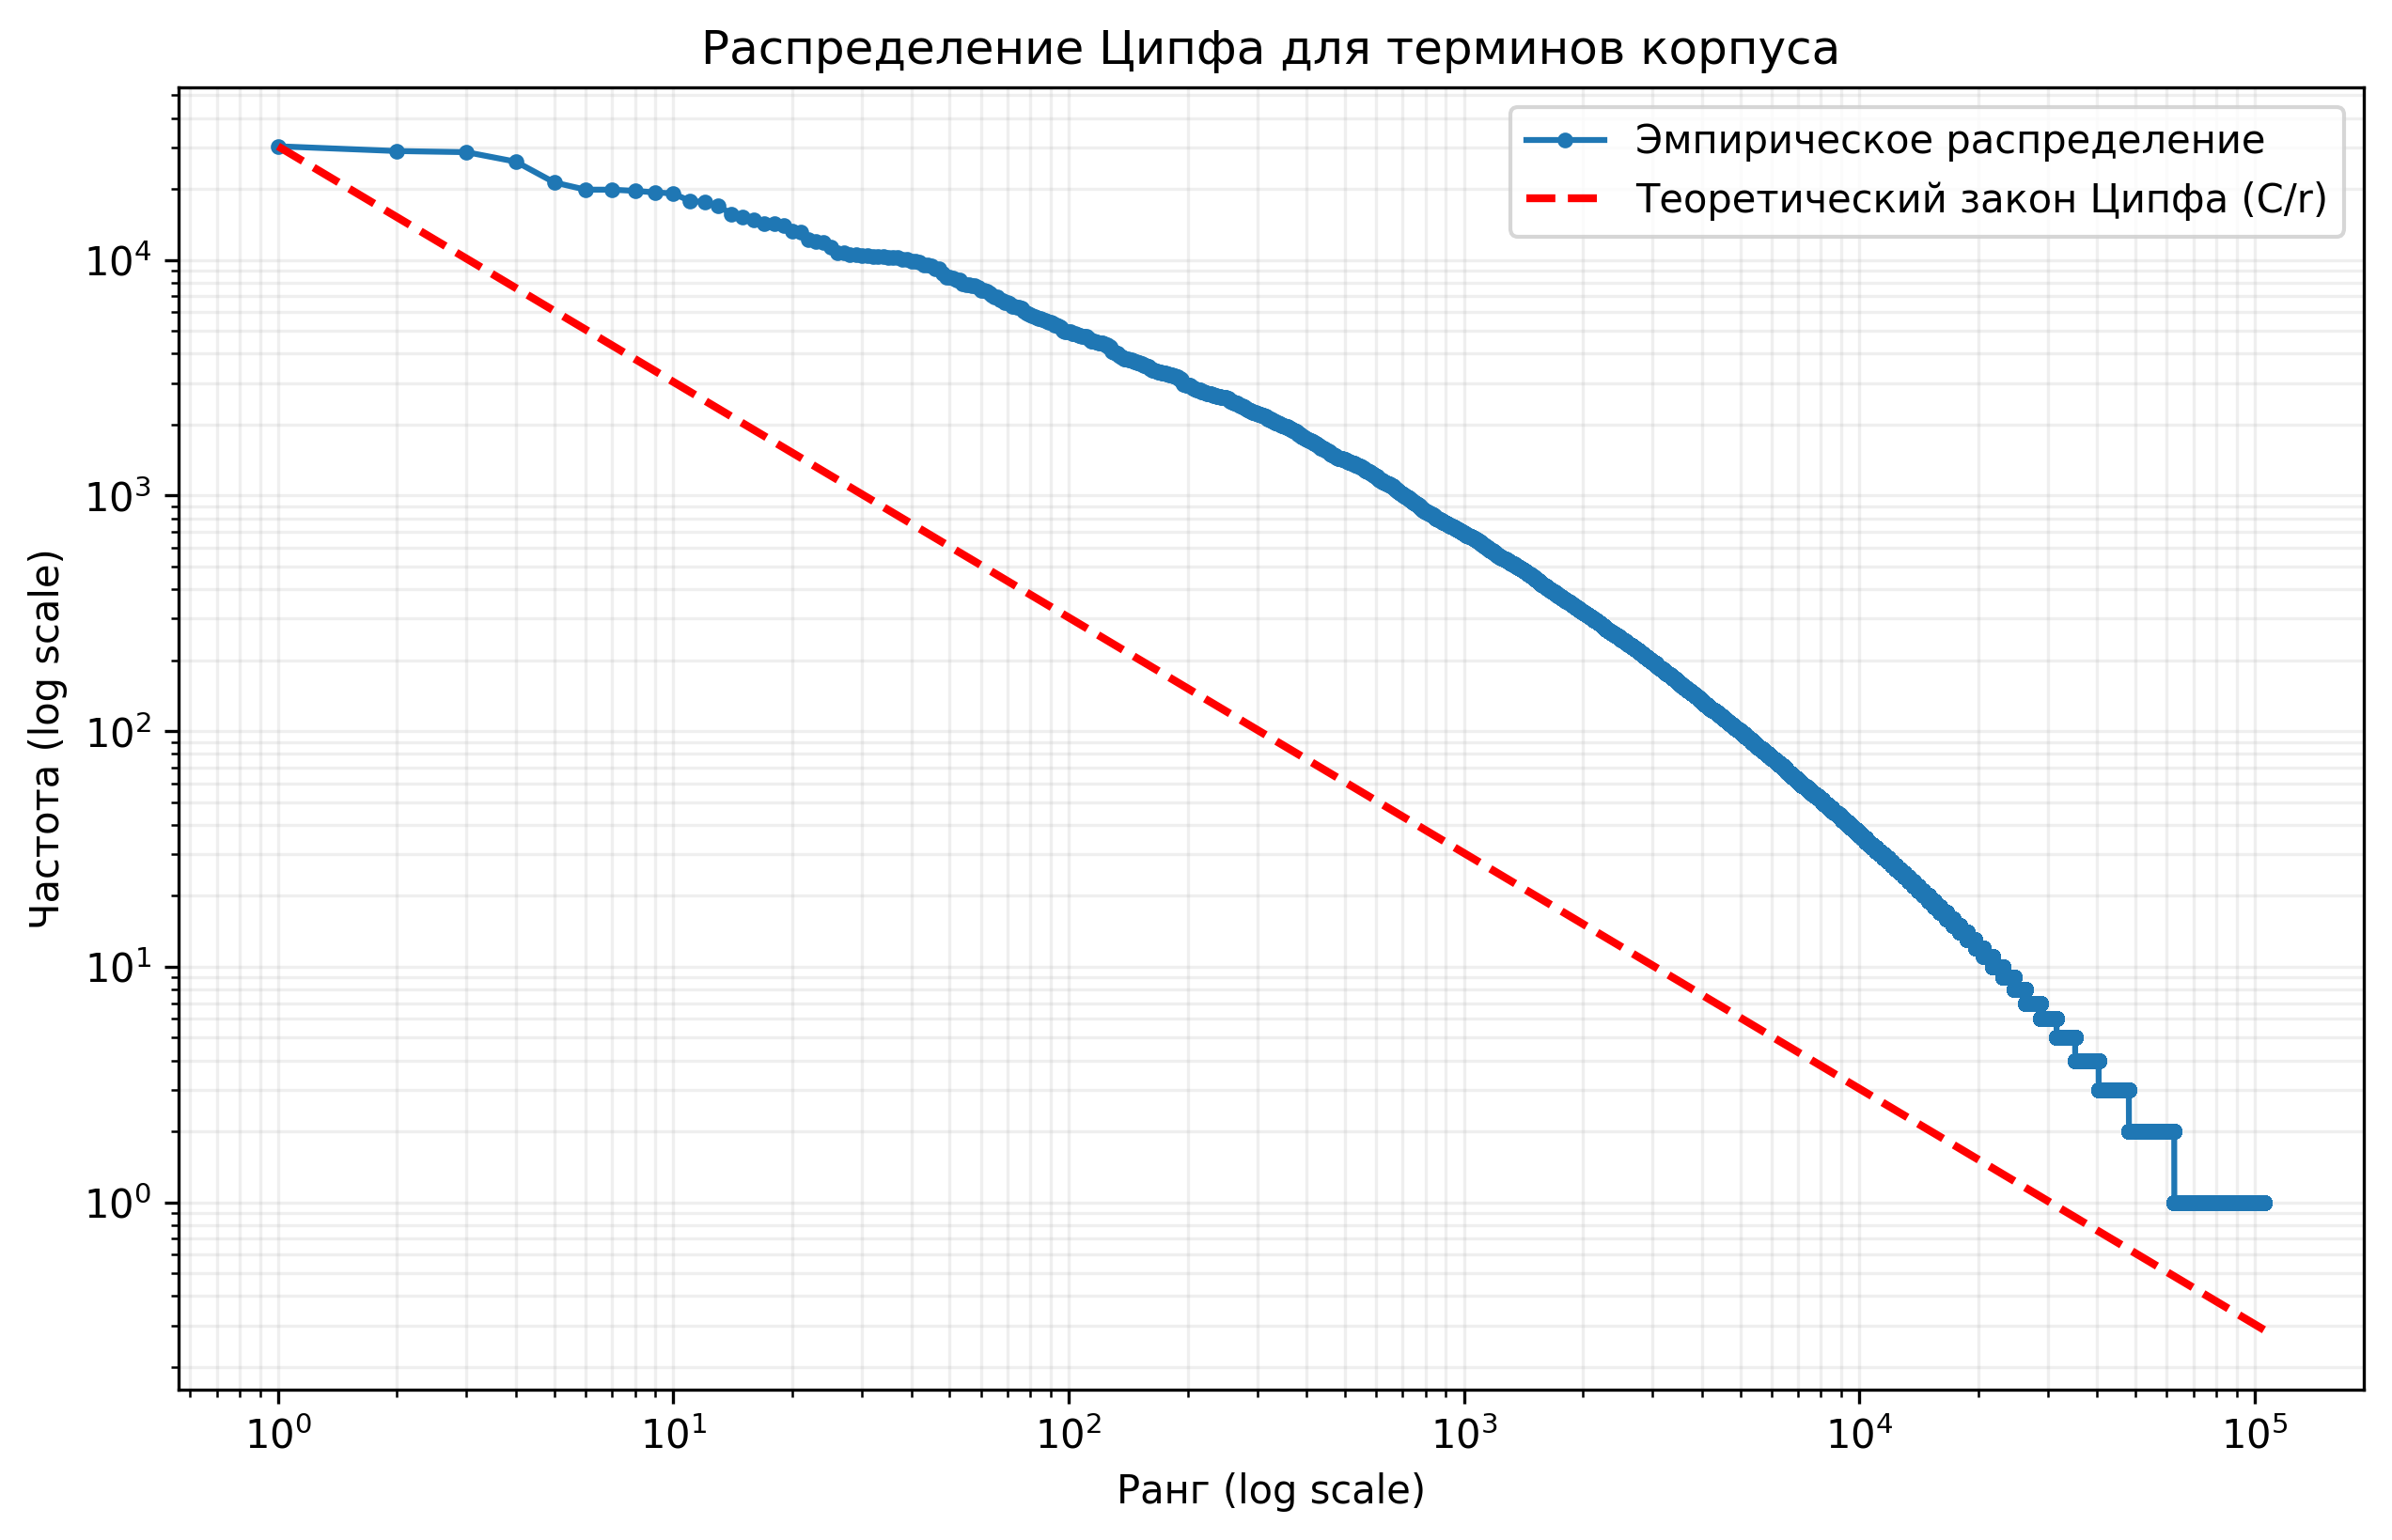
\includegraphics[width=0.9\linewidth]{zipf_distribution.png}
    \caption{Распределение частот терминов в корпусе спортивных новостей}
    \label{fig:zipf}
\end{figure}

Распределение демонстрирует основные характеристики закона Ципфа:
\begin{itemize}
    \item Наиболее частые термины: предлоги и союзы
    \item Средняя часть графика показывает ожидаемую линейную зависимость в логарифмических координатах
    \item Хвост распределения содержит редкие термины, характерные для спортивной тематики
\end{itemize}

Отклонения от идеального закона Ципфа объясняются особенностями корпуса:
\begin{enumerate}
    \item \textbf{Тематическая специфика:} Спортивные новости содержат много терминов, характерных только для этой области ("матч", "гол", "команда", "чемпионат"), что повышает их относительную частоту.
    \item \textbf{Агрессивный стемминг:} Упрощенный стеммер объединяет различные формы слов, что увеличивает частоту основных форм.
    \item \textbf{Структура новостей:} Заголовки и лиды новостей часто содержат одни и те же ключевые слова, что влияет на распределение частот.
\end{enumerate}

\subsection{Тестирование поиска}
Ниже приведены примеры работы программы для различных поисковых запросов.

\textbf{Пример 1. Одиночный запрос}
Запрос: \texttt{футбол}
\begin{verbatim}
Found 4278 document(s) for query: "футбол"

1. Кто сейчас тренирует сборную Италии к Евро-2020 по футболу: Роберто Манчини — крестный отец дебютантов
   URL: https://www.kp.ru/sports/futbol/kto-sejchas-treniruet-sbornuyu-italii-k-evro-2020-po-futbolu
   Source: kp_sport

2. Главный фанат сборной Турции – президент Эрдоган. Он мечтал о карьере футболиста
   URL: https://www.kp.ru/sports/futbol/glavnyj-fanat-sbornoj-turczii-prezident-erdogan
   Source: kp_sport

3. Кто сейчас тренирует сборную Уэльса: Роб Пейдж — заменитель Гиггза
   URL: https://www.kp.ru/sports/futbol/kto-sejchas-treniruet-sbornuyu-uelsa-rob-pejdzh-zamenitel-giggza
   Source: kp_sport

4. Швейцария – столица футбола и спорта. Правительство страны сделало это специально
   URL: https://www.kp.ru/sports/futbol/shvejczariya-stolicza-futbola-i-sporta
   Source: kp_sport

5. Состав сборной Хорватии на Евро-2020 по футболу: шансы и амбиции
   URL: https://www.kp.ru/sports/futbol/sostav-sbornoj-horvatii-na-evro-2020-po-futbolu-shansy-i-ambiczii
   Source: kp_sport

... and 4273 more document(s)
\end{verbatim}


\textbf{Пример 2. Одиночный запрос}
Запрос: \texttt{матч}
\begin{verbatim}
Found 16974 document(s) for query: "матч"

1. Кто сейчас тренирует сборную Уэльса: Роб Пейдж — заменитель Гиггза
   URL: https://www.kp.ru/sports/futbol/kto-sejchas-treniruet-sbornuyu-uelsa-rob-pejdzh-zamenitel-giggza
   Source: kp_sport

2. Швейцария – столица футбола и спорта. Правительство страны сделало это специально
   URL: https://www.kp.ru/sports/futbol/shvejczariya-stolicza-futbola-i-sporta
   Source: kp_sport

3. В Санкт-Петербурге пройдет семь встреч Евро
   URL: https://www.kp.ru/sports/futbol/v-sankt-peterburge-projdet-sem-vstrech-evro
   Source: kp_sport

4. Вундертим – команда Австрии, которой не дали стать чемпионской
   URL: https://www.kp.ru/sports/futbol/vundertim-komanda-avstrii-kotoroj-ne-dali-stat-chempionskoj
   Source: kp_sport

5. Кто сейчас тренирует сборную Нидерландов: Франк де Бур – специалист с ярлыком неудачника
   URL: https://www.kp.ru/sports/futbol/kto-sejchas-treniruet-sbornuyu-niderlandov-frank-de-bur
   Source: kp_sport

... and 16969 more document(s)
\end{verbatim}

\textbf{Пример 3. Булево И (AND)}
Запрос: \texttt{футбол AND матч}
\begin{verbatim}
Found 3171 document(s) for query: "футбол AND матч"

1. Кто сейчас тренирует сборную Уэльса: Роб Пейдж — заменитель Гиггза
   URL: https://www.kp.ru/sports/futbol/kto-sejchas-treniruet-sbornuyu-uelsa-rob-pejdzh-zamenitel-giggza
   Source: kp_sport

2. Швейцария – столица футбола и спорта. Правительство страны сделало это специально
   URL: https://www.kp.ru/sports/futbol/shvejczariya-stolicza-futbola-i-sporta
   Source: kp_sport

3. Состав сборной Хорватии на Евро-2020 по футболу: шансы и амбиции
   URL: https://www.kp.ru/sports/futbol/sostav-sbornoj-horvatii-na-evro-2020-po-futbolu-shansy-i-ambiczii
   Source: kp_sport

4. Кто придумал петь гимны перед матчами
   URL: https://www.kp.ru/sports/futbol/kto-pridumal-pet-gimny-pered-matchami
   Source: kp_sport

5. Турки, сирийцы, афганцы и африканцы – тоже немцы, если речь идет о футболе
   URL: https://www.kp.ru/sports/futbol/turki-sirijczy-afganczy-i-afrikanczy-tozhe-nemczy-esli-rech-idet-o-futbole
   Source: kp_sport

... and 3166 more document(s)
\end{verbatim}

\textbf{Пример 4. Булево ИЛИ (OR)}
Запрос: \texttt{футбол OR матч}
\begin{verbatim}
Found 18081 document(s) for query: "футбол OR матч"

1. Кто сейчас тренирует сборную Италии к Евро-2020 по футболу: Роберто Манчини — крестный отец дебютантов
   URL: https://www.kp.ru/sports/futbol/kto-sejchas-treniruet-sbornuyu-italii-k-evro-2020-po-futbolu
   Source: kp_sport

2. Главный фанат сборной Турции – президент Эрдоган. Он мечтал о карьере футболиста
   URL: https://www.kp.ru/sports/futbol/glavnyj-fanat-sbornoj-turczii-prezident-erdogan
   Source: kp_sport

3. Кто сейчас тренирует сборную Уэльса: Роб Пейдж — заменитель Гиггза
   URL: https://www.kp.ru/sports/futbol/kto-sejchas-treniruet-sbornuyu-uelsa-rob-pejdzh-zamenitel-giggza
   Source: kp_sport

4. Швейцария – столица футбола и спорта. Правительство страны сделало это специально
   URL: https://www.kp.ru/sports/futbol/shvejczariya-stolicza-futbola-i-sporta
   Source: kp_sport

5. Состав сборной Хорватии на Евро-2020 по футболу: шансы и амбиции
   URL: https://www.kp.ru/sports/futbol/sostav-sbornoj-horvatii-na-evro-2020-po-futbolu-shansy-i-ambiczii
   Source: kp_sport

... and 18076 more document(s)
\end{verbatim}
